\chapter{短文本主题模型的数据增强方法研究}\label{chap:Transferring}
\section{引言}
互联网信息媒体的徐梦发展,尤其是微博、小红书、抖音等社交媒体,带来了大量的短文本内容。如何挖掘和理解这些短文本的主题内容是许多领域的重要研究关键研究问题,例如用户兴趣分析、推荐系统和事件检测等\cite{survey_2023}。主题模型是自动将大规模文档集合压缩成内容摘要的模型,其结果表现为一系列相关单词的集合,即潜在主题。传统的主题模型,如非负矩阵分解\cite{NMF}(NMF)和潜在狄利克雷分配\cite{LDA}(LDA)等,在发现长文本中的潜在语义主题结构方面成效显著,但在短文本的应用中面临挑战。因为短文本的词汇数量有限,使得模型中在文档集中寻找单词的共现信息变得困难\cite{survey_2022},这将导致挖掘出噪声较多且缺乏连贯性的主题。

许多研究者致力于解决短文本建模中的数据稀疏性问题。一个简单的策略是使用外部元数据将短文本聚合成更长的伪文本。例如,可以使用标签、作者信息、地点和时间戳等元信息来聚合文本,然后应用LDA进行主题建模\cite{ExTwitter,PoolTwitter}。然而,这些方受限于元数据的信息,可能无法达到预期的效果。同时,这种聚合策略会减少文档数量,从而导致LDA面临文档数量较少这一问题\cite{few_documents}。BICALHO等人\cite{DREx}提出了另一种丰富单词共现模式的方法,即基于分布式表示的文本扩充方法(DREx)。DREx利用词嵌入技术从词汇表中识别相似的词汇,从而将每个短文本扩充为伪长文档。在生成伪文档之后,再对这些文档应用LDA模型。但是,根据词嵌入确定的相似词可能并不具有相同的语义,如多义词等,这将导致原始文档和伪长文档之间出现语义不一致的问题。此外,DREx仅依赖于伪长文档进行主题建模,往往会捕捉到与原始文档不一致的主题。

鉴于现有扩充方法的局限性,本章提出了一种基于提示的短文本数据增强方法。首先,我们提出了一种机制来维持短文本与伪长文本之间的语义一致性。大型语言模型(Large Language Models,LLMs)在近期展示了它们根据文本指令自动生成内容的能力\cite{glm}。受到LLMs想象力和创造力的启发,我们提出了基于提示的文本扩充方法(Instructed-Expansion,IE)。利用可以进行文本自动生成的LLMs,通过指令提示将每个短文本扩充为伪长文档。通过这种新方法,可以将LLMs的知识迁移到短文本主题建模中,而无需采集额外的辅助信息。

其次,虽然大型语言模型(LLMs)可以生成连贯的内容,但由于我们没有在目标数据集上对LLMs进行微调,IE有时会在维持原始文档主题信息的同时,带来一些额外的主题信息。因此,我们提出了一种基于短文本与伪长文本的主题模型(Text-Pairwise Topic Model,TPTM)。其假设短文本与伪长文本是一组成对数据,且短文本中的主题是从其对应伪长文本中的主题中抽取的。这种假设利用了丰富的单词共现性和短文本的独特性,以改进主题建模过程。换而言之,我们提出的TPTM使得IE方法更加灵活且便于使用。

本章工作的主要贡献概括如下:

(1)提出了一种增强短文本数据的方法,即IE方法,利用大型语言模型(LLMs)的知识将每个短文本扩充成伪长文档,用于主题建模。

(2)与以往工作不同,不单是依赖于扩充文档进行LDA主题建模,我们提出了TPTM,将伪长文档与原始短文本作为成对数据同时用于主题建模。

(3)在Tweet、SearchSnippets和StackOverflow数据集上的实验表明,相较于许多基线模型,我们提出的模型能够获得更好的主题质量和分类准确率。

% \section{短文本主题模型的数据增强方法}
% 在本节中,将介绍本章提出的主题建模框架。首先介绍我们提出的基于提示的短文本数据增强方法,它利用大型语言模型生成伪长文本。然后,我们提出了一种基于短文本与伪长文本的主题模型,该模型将伪长文档与原始短文本视为成对数据结合在主题模型中,以得到最终结果。

\section{基于提示的短文本扩充方法}
以往的研究往往将主题模型应用于文本生成这一领域。但在我们中我们采取了相反的方法,将大规模语言模型(Large Language Models,LLMs)用于辅助主题模型在短文本数据集上的建模。
LLMs,如GPT系列模型,是基于深度学习技术的先进自然语言处理工具,它们通过分析大量文本数据来理解和生成语言。这些模型通过在海量数据集上进行训练,能够捕捉到语言的复杂模式和结构,从而在文本生成任务中表现出色。LLMs的核心优势在于其能够生成连贯、有意义且常常难以区分于人类写作风格的文本。在应用方面,LLMs不仅可以高效生成文章、故事和对话,还能够进行内容摘要、自动翻译以及编写代码等。

受到LLMs丰富的想象力和创造力的启发,我们提出了基于提示的短文本数据增强方法(Instructed-Expansion,IE),使用LLMs将每个短文本扩充为一个伪长文本。具体来说,短文本中的词将被用作指导LLMs文本生成的关键词。我们将扩充后的文本称为伪长文档。通过这种方法,可以利用LLMs的外部知识缓解短文本主题建模中遇到的稀疏性问题,而无需除了短文本本身之外的任何额外标签。表\ref{expasion example} 显示了在 Tweet 数据集上,基于 Llama-2-7B\cite{llama2} 进行推断的IE方法示例,记为IE-llama2。在经过预处理后,原始文档包含了词语 "brain fluid buildup delay giffords rehab"。通过使用指令“Generate a text about 100 words based on the following words: ",IE方法获得了一个含有\textit{damage}、\textit{head}、\textit{rehabilitation}等与原文档语义相关的词来讲述故事,从而维持原始文档中的语义并增加了词的共现信息。

我们还对比了现有的另一种扩充方法,基于分布表示的扩充方法(DREx)\cite{DREx}。该方法通过词嵌入扩充短文本,即利用词嵌入计算原数据集词汇表中单词间的相似度,从而为文中单词选择相似度高的词语进行扩充。可以明显观察到我们提出的IE方法和 DREx 之间的差异。在DREx的扩充实例中,我们可以找到一些与原文本语义不相关的词,如“approve”、“push”、“pregnant”等,很难说这些词会与原文本中的单词同属于一个主题。此外,如果我们有两个短文本:“brain fluid buildup”和“pregnant stomach heart”。DREx很可能会将它们扩展为“brain fluid buildup pregnant stomach heart”和“pregnant stomach heart brain fluid buildup”。这两个扩展文本在结果上看是相同的。在某种程度上,这将减少数据集中的文档数量,并使模型认为这些词都属于同一主题。

\begin{table}
    \centering
    \caption{Tweet数据集中的一个文本示例}
    \label{expasion example}
    \adjustbox{width=\textwidth}{
    \begin{tabular}{c|l}
    \hline
    示例 & \multicolumn{1}{c}{文本内容} \\ \hline
    短文本 & brain fluid buildup delay giffords rehab \\ \hline
    \multicolumn{1}{c|}{DREx} & \begin{tabular}[c]{@{}l@{}}brain fluid buildup delay giffords rehab mixture gop supply method pregnant heart approve push \\ reaction process allow excess congresswoman detect technique avoid prevent administration adjourn \\ breathing mind halt plan require strain move liver contain force heat amount hearing rehabilitation \\ clinton affect memory announcement cause change vote stomach ongoing response scan\end{tabular} \\ \hline
    \begin{tabular}[c]{@{}c@{}}IE-llama2\end{tabular} & \begin{tabular}[c]{@{}l@{}}The brain is a complex organ that is susceptible to damage after a traumatic event such as a\\ shooting. When a bullet hits the brain, it can cause bleeding and swelling, leading to a buildup of \\fluid in the affected area. This buildup can cause delays in the healing process and can lead to further\\ damage if left untreated. In the case of former Congresswoman Gabrielle Giffords, her shooting in \\ 2011 caused significant damage to her brain, leading to a long and difficult rehabilitation process. \\Despite the challenges, Giffords has made remarkable progress and is now able to communicate and\\ function independently.
    \end{tabular} \\ \hline
    \end{tabular}
    }
\end{table}

\section{基于成对文本的主题模型}
本节首先给出一些定义。给定一个包含$D$个文档的短文本语料库$\mathbb{S}=\{S_d\}_{d=1}^D$和一个词汇表$W=\{w_1,w_2,\dots,w_V\}$。可以为$\mathbb{S}$中的每个实例使用IE方法生成一个伪文档,从而得到大小为$D$的伪文档语料库$\mathcal{P}$,表示为$\mathbb{P}=\{P_d\}_{d=1}^D$。将包含原文档和伪文档的整个数据集表示为$\mathbb{D}=\{S_d,P_d\}_{d=1}^D$。每个短文本的格式为$S_d=\{w_{d,1},w_{d,2},\dots, w_{d,M_d}\}$,其中$w_{d,n}$是$S_d$中的第$n^{th}$个词,$M_d$是$S_d$中的词数。因此,伪长文档$P_d$具有与$S_d$相同的格式,即$P_d=\{w_{d,1},w_{d,2},\dots, w_{d,N_d}\}$,其中$N_d$是$P_d$中的词数。数学符号在表\ref{notations}中解释。

\begin{table}
    \centering
    \caption{在本章涉及的数学符号及其说明}
    \label{notations}
    \adjustbox{width=0.65\textwidth}{
    {\begin{tabular}{cc}
    \toprule
    数学符号 & 说明\\
    \midrule
    $K$& 主题数量 \\
    $D$ & 短文本语料库的文本数量\\
    $V$ & 语料库中的词表长度\\
    $\mathcal{S}$ & 短文本语料库$\mathcal{S}=\{S_d\}_{d=1}^D$\\
    $\mathcal{P}$ & 伪长文本语料库$\mathcal{P}=\{P_d\}_{d=1}^D$\\
    $\mathcal{D}$ & 整个语料库$\mathbb{D}=\{S_d,P_d\}_{d=1}^D$\\
    $N_d$ & 伪长文本$P_d$包含的单词数\\
    $M_d$ & 短文本$S_d$包含的单词数\\
    $\vec\beta_k$ & 主题$k$对应的主题-词分布\\
    $\vec\eta$ & $\beta_k$的狄利克雷先验值\\
    $\vec\theta_d$ & 伪长文本$P_d$对应的文档-主题分布\\
    $\vec\alpha$ & $\theta_d$的狄利克雷先验值\\
    $z_{d,n}$ & 短文本$S_d$中第$n$个单词对应的主题编号\\
    $z_{d,n}^+$ & 伪长文本$P_d$中第$n$个单词对应的主题编号\\
    $\boldsymbol{\vec l}$ & 语料库$\mathcal{D}$中的所有单词对应的主题,$\boldsymbol{\vec l}=\{\boldsymbol{\vec z}_d^+,\boldsymbol{\vec z}_d\}_{d=1}^D$\\
    $n_{P_d}^{(k)}$ & $P_d$中属于主题$k$的单词数 \\
    $n_{S_d}^{(k)}$ & $S_d$中属于主题$k$的单词数 \\
    $n_k^{(v)}$ & 在整个语料库$\mathcal{D}$中属于主题$k$的单词数\\
    \bottomrule
    \end{tabular}}}
\end{table}

我们提出了基于成对文本的主题模型(Text-Pairwise Topic Model,TPTM)。TPTM不仅利用了伪长文档中丰富的词共现信息,还考虑了原始短文本中的内在主题。由于$S_d$和$P_d$是一一对应的,TPTM假设每个短文本$S_d$中的主题来自其对应的伪文档$P_d$。类比于新闻报道与其标题的关系,新闻标题一定体现了其报道内容的主题内容。TPTM对于短文本的生成过程可以分为两个阶段描述。第一阶段遵循LDA模型的假设来生成扩充语料库$\mathcal{P}$。在第二阶段,$S_d$中的每个词都是通过首先从$P_d$中已有的主题中采样一个主题$z$,然后从$\vec\beta_z$中采样一个词来生成的。TPTM的概率图模型如图\ref{TPTM_graph}所示,其中$\vec \alpha$和$\vec\eta$是狄利克雷先验。TPTM具体的生成过程描述如下:

\pagebreak

\begin{itemize}[]
    \item[(1)] 对于每一个主题 $k\in {1,\dots,K}$:
    \begin{itemize}
        \item[(a)] 采样一个主题-词分布 $\vec\beta_k\sim \mbox{Dirichlet}(\vec\eta)$ 
    \end{itemize}
    \item[(2)] 对于扩充后得到的每一篇伪长文本 $P_d \in \mathcal{P}$:
    \begin{itemize}
        \item[(a)] 采样一个文档-主题分布 $\vec\theta_d\sim \mbox{Dirichlet}(\vec\alpha)$
        \item[(b)] 对于 $P_d$ 中的每个单词 $w_{n}^+$:
        \begin{itemize}
            \item[i.] 采样一个主题 $z^+\sim \mbox{Multinomial}(\vec\theta_d)$
            \item[ii.] 采样一个单词实体 $w_{n}^+\sim \mbox{Multinomial}(\vec\beta_{z^+})$
        \end{itemize}
    \end{itemize}
    \item[(3)] 对于原来的每一篇短文本 $S_d \in \mathcal{S}$:
    \begin{itemize}
        \item[(a)] 对于 $S_d$ 中的每个单词 $w_{n}$:
        \begin{itemize}
            \item[i.] 从$P_d$的主题$\{z_{d,n}^+\}_{n=1}^{N_d}$中采样一个主题$z$
            \item[ii.] 采样一个单词实体$w_{n}\sim \mbox{Multinomial}(\vec\beta_z)$
        \end{itemize}
    \end{itemize}
\end{itemize}

\begin{figure}[ht]
    \centering
    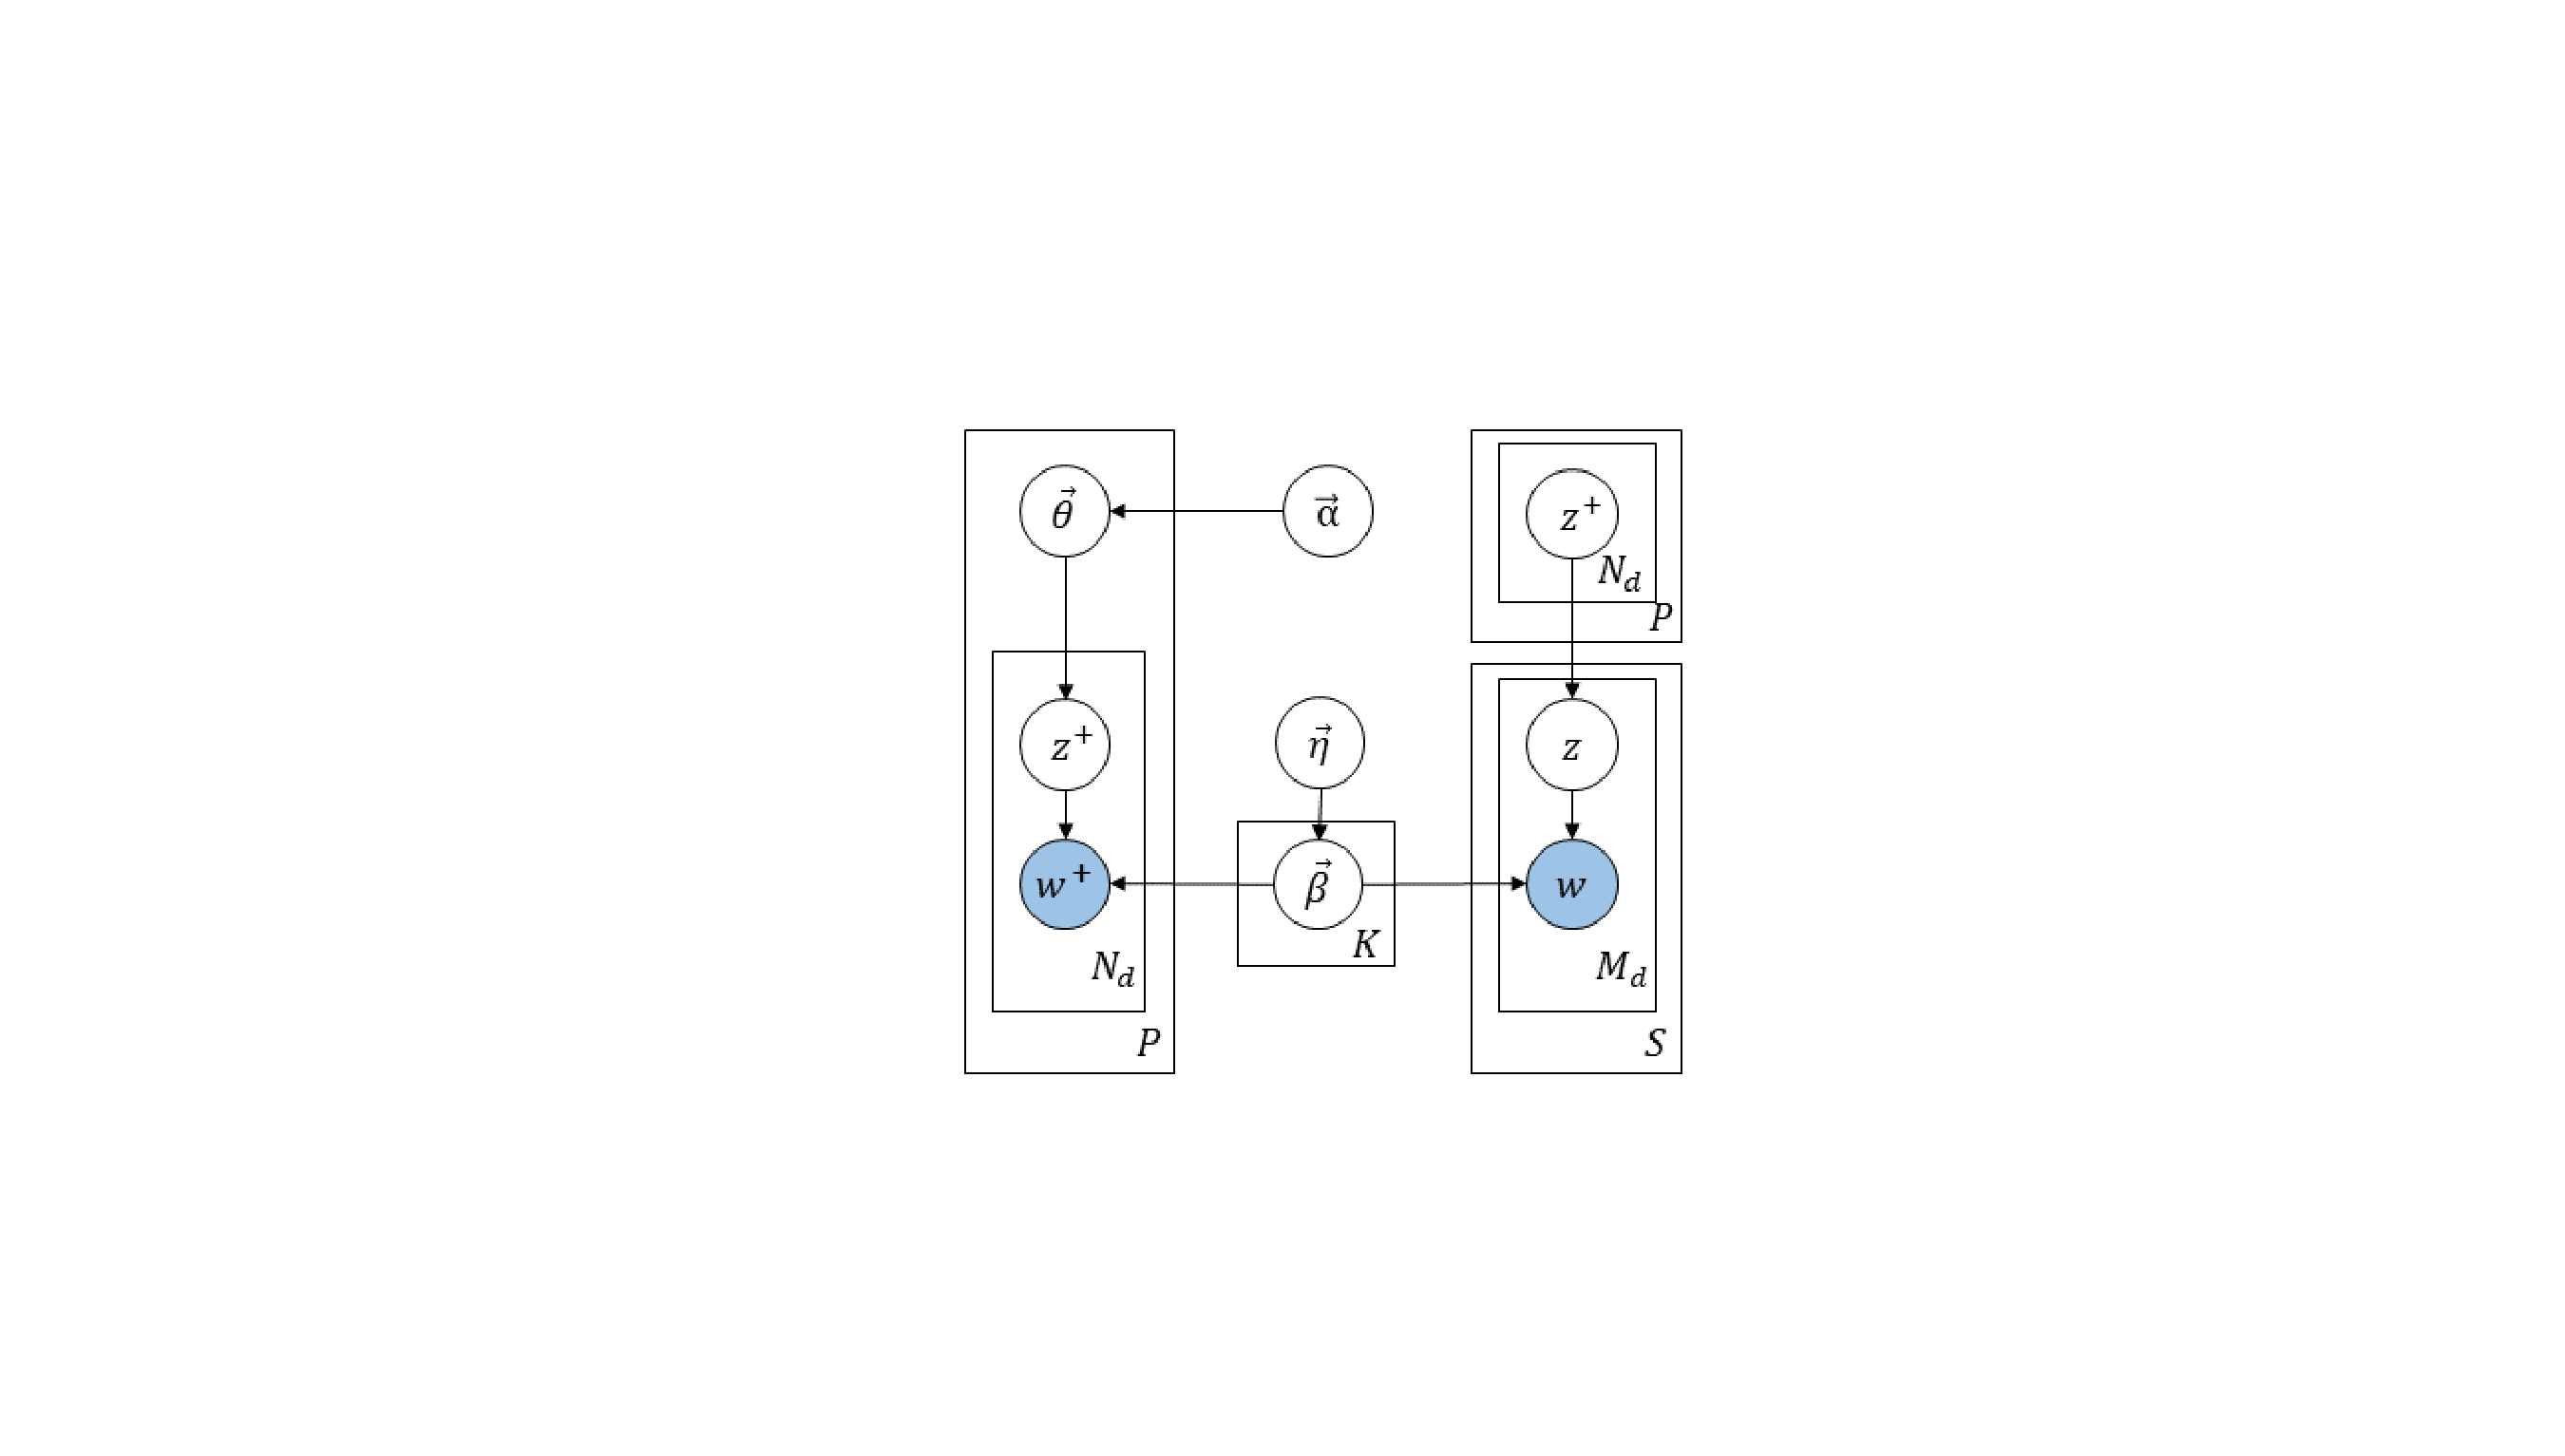
\includegraphics[trim= 15cm 5cm 15cm 5cm, clip=true, width=0.5\textwidth]{chap3/IETM.eps}
    \caption{基于成对文本的主题模型(TPTM)的概率图模型} 
    \label{TPTM_graph}
\end{figure}

\section{模型推断}
给定语料库$\mathbb{S}$和扩充语料库$\mathbb{P}$之后,需要推导出生成模型的后验分布。然而,精确的后验分布推断是不可求解的。同大部分主题模型一样,我们采用吉布斯采样算法进行后验推断。根据图\ref{TPTM_graph}中的基于成对文本的主题模型生成模型,通过对$\theta$和$\beta$进行积分,可以得到每个词对应主题的条件后验概率分布,以执行推断过程。吉布斯采样算法的详细细节可以在算法\ref{Gibbs_algo}中找到。图\ref{OverallFramework}中描绘了主题的采样过程。在每次迭代中,对于一篇伪长文档,将根据当前的主题-词分布以及这一篇文档对应的主题分布,为每个词采样一个主题。然后,为短文本中的每个词,通用利用当前的主题-词分布,从出现在其对应伪长文档中的主题中采样一个主题。

\begin{figure}[ht]
    \centering
    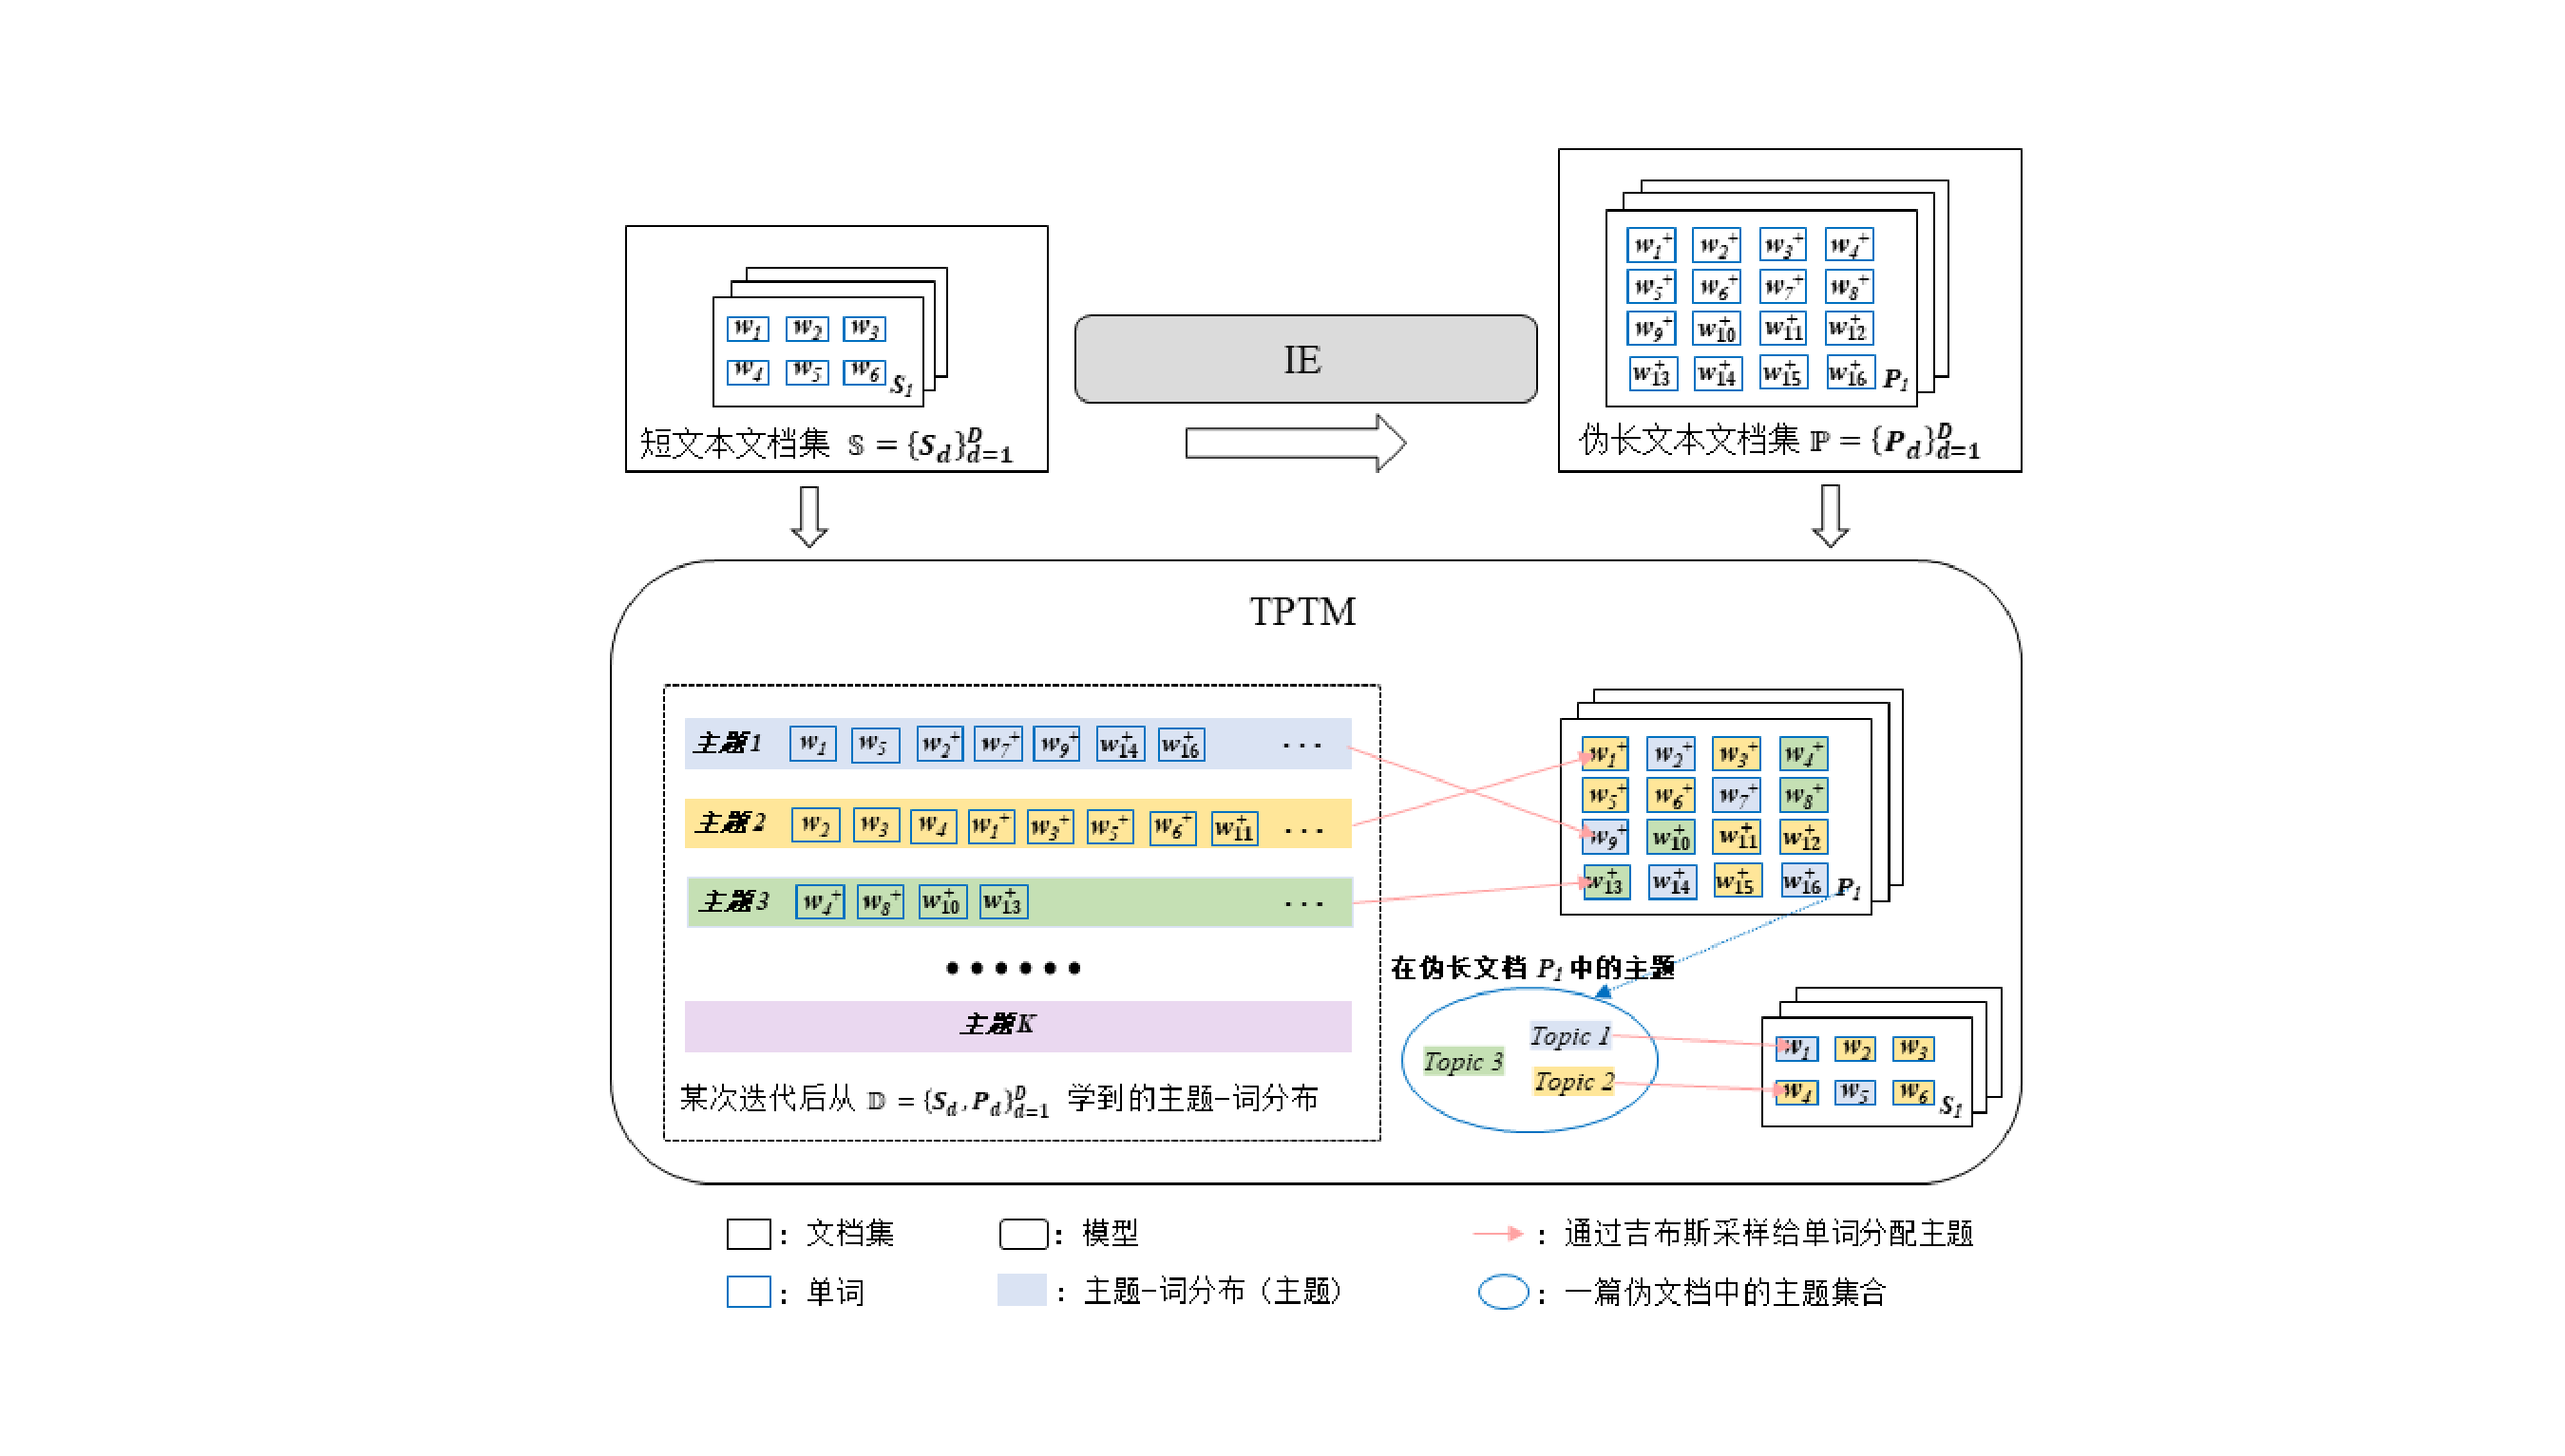
\includegraphics[trim= 10cm 2cm 8cm 2cm, clip=true, width=\textwidth]{chap3/Structure.eps}
    \caption{整体框架示意图} 
    \label{OverallFramework}
\end{figure}

\begin{algorithm}[tb]
    \caption{TPTM的吉布斯采样过程}
    \label{Gibbs_algo}
    \LinesNumbered
    \KwIn{$K$, $\alpha$, $\eta$, 文档集 $\mathcal{S}$, $\mathcal{P}$ 以及迭代次数 $I$}
    \KwOut{主题分配 $\vec{z}$ 和 $\vec{z}^+$; 主题-词的后验分布 $\beta$}
    随机初始化 $\vec{z}^+$\;
    根据 $\vec{z}^+$ 随机初始化 $\vec{z}$ \;
    初始化计数变量 $n_{P_d}^{(k)}$, $n_{S_d}^{(k)}$, $n_k^{(v)}$\;
    \For{第$i$次迭代, $i\in 1,2,\dots,I$}{
    \For{伪长文档$P_d$,$P_d\in \mathcal{P}$}{
    \For{$P_d$中的每一个单词, $w_{d,n}^+\in P_d$}{
    根据Eq.(\ref{sample1})采样一个主题$z_{d,n}^+$分配给单词$w_{d,n}^+$\;
    }
    }
    \For{短文本$S_d$,$S_d\in \mathcal{S}$}{
    \For{$S_d$中的每一个单词,$w_{d,n}\in S_d$}{
    根据Eq.(\ref{sample2})采样一个主题$z_{d,n}$分配给单词$w_{d,n}$\;
    }
    }
    }
\end{algorithm}

在吉布斯采样过程中,我们需要求解TPTM两个条件后验概率分布:(1)为伪文档$P_d$中的词$w_{d,n}^+$采样一个主题$z_{d,n}^+$的条件后验概率分布;(2)对于原始文档$S_d$中的词$w_{d,n}$,将采样一个主题$z_{d,n}$条件后验概率分布。推导过程与细节见附录A。
对于(1),我们有
\begin{equation}
\label{sample1}
\begin{aligned}
    &p(z_{d,n}^+=k|\boldsymbol{\vec l}_{\neg(P_{d,n})},\mathcal{D})\propto\\
    &\frac{n_{k,\neg(P_{d,n})}^{(v)}+\eta}{\sum_{i=1}^V(n_{k,\neg(P_{d,n})}^{(i)}+\eta)}
    \cdot\frac{n_{P_d,\neg(P_{d,n})}^{(k)}+\alpha}{N_d-1+K\alpha}\cdot\left(\frac{N_d-1}{N_d}\cdot\frac{n_{P_d,\neg(P_{d,n})}^{(k)}+1}{n_{P_d,\neg(P_{d,n})}^{(k)}}\right)^{n_{S_d}^{(k)}}
    \end{aligned}
\end{equation}
其中$\boldsymbol{\vec l}=\{\boldsymbol{\vec l}_d\}_{d=1}^D=\{\boldsymbol{\vec z}^+, \boldsymbol{\vec z}\}=\{\boldsymbol{\vec z}_d^+,\boldsymbol{\vec z}_d\}_{d=1}^D$。$n_{P_d}^{(k)}$ 和 $n_{S_d}^{(k)}$ 分别是第 $d$ 个伪文档和原始文档中属于第 $k$ 个主题的词的数量。而 $n_k^{(v)}$ 是分配给 $\mathcal{D}$ 中第 $k$ 个主题的词 $v$ 的出现次数。所有带有 $\neg\bullet$ 的计数表示排除来自 $\bullet$ 的计数。

类似地,对于(2),原始文档$S_d$中的词$w_{d,n}$,其采样一个主题$z_{d,n}$的条件后验概率分布为公式(\ref{sample2})为
\begin{equation}
    \begin{aligned}
    \label{sample2}
    p(z_{d,n}=k|\boldsymbol{\vec l}_{\neg(S_{d,n})},\mathcal{D})
    \propto\frac{n_{k,\neg(S_{d,n})}^{(v)}+\eta}{\sum_{i=1}^V(n_{k,\neg(S_{d,n})}^{(i)}+\eta)}\cdot\left(\frac{n_{P_d}^{(k)}}{N_d}\right)
    \end{aligned}
\end{equation}

显然,在这两个采样方程中,将伪文档作为辅助信息有助于提高短文本的主题学习。另一方面,我们还通过使用来自相应短文本的信息来增强伪文档的主题学习。此外,在采样迭代过程中,$n_{P_d,\neg(P_{d,n})}^{(k)}$ 可能等于零。当 $n_{P_d,\neg(P_{d,n})}^{(k)}=0$ 时,我们将公式(\ref{sample1})中的第三项设为1。

TPTM在一次迭代中需要为整个语料库$\mathcal{D}$中的每一个词都采样一次主题,所以TPTM的时间复杂度为$O(KW)$,其中$K$是主题数,$W$是整个语料库$\mathcal{D}$中的总词数。可以看出TPTM有着与LDA模型相同的时间复杂度。经过吉布斯采样迭代后,我们可以估计主题-词分布$\vec{\beta}_k$,如公式(\ref{beta})所示,从而获得最终的潜在主题。

\begin{equation}
    \label{beta}
    \beta_{k,v}=\frac{n_k^{(v)}+\eta}{\sum_{i=1}^V(n_k^{(i)}+\eta)}
\end{equation} 

\section{讨论}
TPTM利用短文本和伪文档之间存在的单词共现模式来挖掘主题。因此,TPTM在很大程度上缓解了短文本中单词共现信息的不足。另一种提高短文本建模性能的可行方法是仅依赖扩充后的伪文档来训练LDA模型。然而,由于原始文档和伪文档之间可能存在的不一致性,这种方法可能会忽略甚至消除短文本中的独特信息。与此相反,TPTM将原始文档和其伪文档视为两个不同但几乎具有相同语义的数据集进行主题挖掘。

TPTM从扩展文档中抽取主题的思想是新颖的。不过,TPTM的概率图模型结构类似于自聚合主题模型(SATM)\cite{SATM}。在标准主题建模中,SATM假设每个短文本都是从一个未观察到的长伪文档中抽样得来的,并从中推断出潜在主题。相反,在本文中,我们可以获得用于主题建模的每个伪文档的具体内容。此外,SATM直接从伪文档中的词汇中抽样短文本中的词汇,而TPTM首先为短文本抽样主题,然后从主题-词分布中抽样词汇。因此,TPTM放宽了SATM中的假设,使其在建模短文本时更加合理和灵活。

此外,我们希望探讨TPTM与COTM\cite{COTM}之间的相似性和差异性。COTM是为建模短文本而设计的,这些短文本的特点是它们与通常较长的普通文档共现。例如,一个新闻文章后面可能跟着多条用户评论。因此,COTM是一种一对多的模型,并且短文本中的内容可能与其对应的普通文档讨论不同的主题。然而,在TPTM中,通过Instructed-Expansion方法,可以获得与原始文档几乎完全相同语义的伪文档。由于TPTM是一对一的模型,我们不必担心这原语料库与伪文档语料库之间的语义不一致。更重要的是,许多短文本模型的难点在于缺乏与它们对应的普通文档或辅助信息。但在本文中,我们可以通过大型语言模型(LLMs)生成伪文档,并使用TPTM更好地建模原始语料库与扩展语料库之间的关联。

\section{实验设置}
本节基于现实生活中的短文本数据集,同许多短文本主题模型一起进行了一系列的实验,以评估本章提出的短文本扩充方法及主题模型的有效性。

\subsection{数据集}
本章采用了三个真实的短文本数据集进行实验分析,分别是:(1)Tweet\cite{GSDMM}数据集,包含2,472个推文,涵盖了89个类别;(2)SearchSnippets数据集,包含来自8个不同领域的网络搜索片段\cite{SearchSnippets}。(3)StackOverflow数据集,包含从20个不同领域的问题中随机选择的20,000个问题的标题\cite{SearchSnippets}。

对于所有数据集,我们进行了以下预处理步骤:(1)将字母转换为小写;(2)去除非拉丁字符和停用词;(3)利用NLTK的WordNet词形还原器的单词进行词干提取;(4)过滤掉长度小于2的短文本。我们采用GPT-3.5(text-davinci-003)\cite{GPT3}、配置了Low-Rank Adaptation(LoRA)\cite{lora} 的Llama-7b\cite{llama}, 以及Llama2-7b-chat\cite{llama2},应用于我们提出的Instructed-Expansion方法,分别记为IE-GPT、IE-llama和IE-llama2。使用指令:“Generate a text about 100 words based on the following words:”,并结合预处理后的短文本中的词汇,我们获得了扩展后的伪文档数据集。对于伪文档数据集,还有一个额外的预处理步骤,即移除不在原始语料库中的单词。每个数据集预处理后的统计数据汇总在表\ref{TableCopusInformation}中,其中$D$代表每个数据集中的文档数量,$V$表示词汇表的大小,$C$指数据集中的类别数量,$N$表示语料库中文本的平均长度。最后三行是不同大模型得到的伪长文档集的平均长度。

\begin{table}
    \centering
    \caption{数据集的基本信息}
    \label{TableCopusInformation}
    \adjustbox{width=0.55\textwidth}{
        \begin{tabular}{lccc}
        \hline
        数据集  & Tweet & SearchSnippets & StackOverflow \\ \hline
        $D$        & 2,472  & 12,295          & 16,407         \\
        $V$        & 4,758  & 3,803           & 1,682          \\
        $C$        & 89    & 8              & 20            \\
        短文本-$N$ & 8.5   & 14.4           & 4.8           \\
        IE-GPT-$N$   & 44.1  & 47.1           & 49.2          \\
        IE-llama-$N$ & 40.3  & 43.4           & 49.2          \\
        IE-llama2-$N$   & 42.4     & 50.9        & 38.7        \\\hline
        \end{tabular}
        }
\end{table}

\subsection{对比模型}
为了验证我们提出的短文本主题模型的有效性,本节将所提出的模型与多种现有模型进行对比并根据评价指标来分析结果,参与对比的模型有(1)LDA模型; (2)基于DMM的模型:DMM模型、GPUDMM模型、MultiKE-DMM模型和TSSE-DMM模型;(3)基于文本自聚合的模型:PTM模型和PYSTM模型;(4)BTM模型和SeaNMF模型。对比模型的详细介绍如下:

\textbf{(1)LDA\cite{LDA}:}该方法以狄利克雷分布作为先验分布,将每个文档视为主题的概率分布,每个主题则视为词汇的概率分布,通过推断这些分布的后验分布来揭示文档的潜在主题内容。

\textbf{(2)DMM\cite{GSDMM}:}该模型假设每篇文档由单一主题生成。它基于Dirichlet分布指派文档至特定主题,并通过多项分布来确定该主题下的词汇分布,从而揭示文档的主要主题。

\textbf{(3)GPUDMM\cite{GPUDMM}:}该模型是基于外部知识的方法,利用广义波利亚罐模型将词向量引入DMM模型中,以增强DMM模型的主题挖掘能力

\textbf{(4)MultiKE-DMM\cite{MKEDMM}:}引入词向量与知识图谱两种外部知识,构建多知识加权的词表示向量,并利用多知识融合的度量方法来捕捉单词更全面的相互关系。

\textbf{(5)TSSE-DMM\cite{TSSE}:}通过语义增强机制,提高模型对短文本中稀疏特征的处理能力,从而更有效地识别和区分主题。

\textbf{(6)PTM\cite{PTM}:}该模型将相关的短文本组合成一个较长的伪文档,以隐式地增加数据的丰富性和上下文信息,从而改善主题模型在处理短文本时的表现和准确性。

\textbf{(7)PYSTM\cite{PYSTM}:}该模型通过从Dirichlet过程中采样来参数化PTM模型中伪长文本的数量,能够灵活地考虑多少短文本是出自于一个伪长文本。

\textbf{(8)BTM\cite{BTM}:}该模型基于“biterms”(文档中词对的集合)而非整个文档或单个词来建模,从而直接捕捉词汇间的共现模式。

\textbf{(9)SeaNMF\cite{SeaNMF}:}该模型通过非负矩阵分解,将短文本集的上下文语义和词嵌入信息引入模型中。

\subsection{参数设置}
所有基准模型的参数值都按照其作者在论文中的推荐值设置。我们为TPTM选择了$\alpha=1.0$ 和 $\beta=0.01$。同时将所有对比模型的迭代次数设定为2,000次。 每个模型在每个数据集上都会运行5次,并记录其平均值作为最终结果。由于主题建模是一种无监督学习方法,对于主题数的设置没有一个很好的参考。在本节中,实验中所有模型的主题数量都设定为$K=25, 50$。

\subsection{评估指标}
为了对实验结果进行评估,我们专注于两个常用的评估指标:主题一致性和主题多样性。主题一致性是衡量主题可解释性的定量指标。在计算主题一致性时,需要使用外部数据集来根据术语共现为词对打分。我们采用标准化点互信息(Normalized Pointwise Mutual Information,NPMI)\cite{coherence} 来评估模型所挖掘出的主题在外部的语料库(英文维基百科文章)上的主题一致性。NPMI 暗示了一个主题的最可能单词倾向于在同一文档中共同出现。给定一个主题 $k$ 及其概率最高的前 $T$ 个单词 $(w_1,w_2,\dots,w_T)$,主题 $k$ 的 NPMI 为:
\begin{equation}
    \mbox{NPMI}(k)=\sum_{j=2}^T\sum_{i=1}^{j-1}-\frac{\log\frac{P(w_i,w_j)}{P(w_i)P(w_j)}}{\log P(w_i,w_j)}
 \end{equation}
其中 $p(w_i)$ 是单词 $w_i$ 出现在文档中的概率,$p(w_i,w_j)$ 是单词 $w_i$ 和 $w_j$ 同时出现在同一文档中的概率。NPMI数值越大意味着一个主题中的单词倾向于在同一文档内共同出现。本节计算所有主题前5、10和15个词的NPMI平均值作为最终结果。

主题多样性对应于每个词在同一模型的其他主题中出现的平均概率\cite{DVAE}。本节对所有主题的前15个词使用主题独特性(Topic Unique,TU)进行度量\cite{TU}。对于主题 $K$ 的前 $T$ 个单词,它被定义为
\begin{equation}
    TU(k) = \frac{1}{T}\sum_{i=1}^T\frac{1}{cnt(w_i)}
\end{equation}
其中 $cnt(w_i)$ 是单词 $w_i$ 在所有主题的前 $T$ 个单词中出现的总次数。TU接近1表示主题更加多样化,接近0则表示这个主题重复出现,是冗余的。

直观上,较高的NPMI通常会导致较低的TU,因为一致的主题倾向于被重复发现,而较高的TU则会带来较低的NPMI,因为其鼓励发现更多边缘主题\cite{NQTM}。因此,我们更倾向于在上述两个方面之间取得良好平衡的主题。为了衡量这一点,与Adji等人\cite{overallQuality,iclr/0003G0ZTCZ22}相同,我们采用了主题质量(Topic Quality,TQ)分数作为总体评估的指标,该得分被定义为NPMI和TU值的乘积,$\mbox{TQ}=\mbox{NPMI}\times \mbox{TU}$。%对于所有指标,$t$检验显示SpareNTM与每个基线之间的性能差异在平均值方面是否具有统计学显著性。如果从$t$检验中得到的$P$值低于0.05,我们认为成对性能差异是显著的。

\section{实验结果与分析}
\label{experiment_r}

\subsection{主题质量评估}
本节将TPTM的实验结果与其他基线模型进行对比分析。TPTM-GPT、TPTM-llama和TPTM-llama2分别代表使用IE-GPT、IE-llama和IE-llama2的TPTM。如表\ref{TableTopicQuality50}和\ref{TableTopicQuality100}所示,可以观察到,我们提出的TPTM-llama2在所有三个数据集中几乎都取得了最佳的主题质量(TQ)得分。这验证了TPTM-llama2在主题一致性和多样性之间达到了比其他基线更好且更均衡的主题质量。从表\ref{TableTopicQuality50}和表\ref{TableTopicQuality100}也可以看到,DREx相比于其他基线模型获得了最佳的主题质量,尤其是在NPMI方面。由于DREx通过使用词嵌入来选择词汇表中的相似词来扩展短文本,所以相似词共享相同主题这一点是直观的,这确实提高了主题一致性。不幸的是,DREx容易产生重复主题。这是因为DREx会模糊主题之间的区别。例如,如果我们有两个短文本:“brain fluid buildup”和“pregnant stomach heart”,我们不能简单地将这些词视为属于同一主题。然而,DREx可能会将它们扩展为“brain fluid buildup pregnant stomach heart”和“pregnant stomach heart brain fluid buildup”。这两个扩展文本在结果上看是相同的。在某种程度上,这将减少数据集中的文档数量,并使模型认为这些词都属于同一主题。此外,在基于DMM的模型中,GPUDMM和MultiKE-DMM因为使用了外部知识取得了更好的结果。基于上述分析,可以证明本文提出的TPTM成功地通过从LLMs转移知识,为短文本数据集挖掘出了更高质量的潜在主题。

\begin{table}[ht]
    \centering
    \caption{当主题数为25时的主题质量,其中加粗表示最好的结果}
    \label{TableTopicQuality50}
    \adjustbox{width=0.85\textwidth}{
    \begin{tabular}{lccc|ccc|ccc}
    \hline
    \multicolumn{1}{c}{\multirow{2}{*}{模型}} & \multicolumn{3}{c|}{Tweet} & \multicolumn{3}{c|}{SearchSnippets} & \multicolumn{3}{c}{StackOverflow} \\
    \multicolumn{1}{c}{} & NPMI & TU & \textbf{TQ} & NPMI & TU & \textbf{TQ} & NPMI & TU & \textbf{TQ} \\\hline
    LDA         & 0.187          & 0.872          & 0.163          & 0.234          & 0.799          & 0.187          & 0.212          & 0.592          & 0.126          \\
    BTM         & 0.186          & 0.758          & 0.141          & 0.245          & 0.668          & 0.164          & 0.196          & 0.357          & 0.070          \\
    SeaNMF      & 0.178          & \textbf{0.966} & 0.172          & 0.250          & 0.776          & 0.194          & 0.199          & 0.605          & 0.120          \\
    DMM         & 0.191          & 0.822          & 0.157          & 0.244          & 0.675          & 0.165          & 0.195          & 0.430          & 0.084          \\
    GPUDMM      & 0.196          & 0.751          & 0.147          & 0.25           & 0.725          & 0.183          & 0.201          & 0.360          & 0.072          \\
    TSSE-DMM    & 0.198          & 0.714          & 0.141          & 0.225          & 0.569          & 0.128          & 0.188          & 0.457          & 0.086          \\
    MultiKE-DMM & 0.190          & 0.792          & 0.150          & 0.219          & 0.745          & 0.163          & 0.163          & 0.418          & 0.068          \\
    PTM         & 0.184          & 0.813          & 0.150          & 0.240          & 0.772          & 0.185          & 0.211          & 0.577          & 0.122          \\
    PYSTM       & 0.184          & 0.853          & 0.157          & 0.233          & 0.851          & 0.198          & 0.195          & 0.725          & 0.141          \\
    DREx        & \textbf{0.262} & 0.793          & \textbf{0.207} & \textbf{0.283} & 0.744          & 0.210          & \textbf{0.279} & 0.586          & 0.163          \\\hline
    TPTM-GPT    & 0.223          & 0.818          & 0.182          & 0.252          & 0.889          & 0.224          & 0.242          & 0.727          & 0.176          \\
    TPTM-llama  & 0.216          & 0.905          & 0.195          & 0.246          & \textbf{0.965} & \textbf{0.237} & 0.224          & \textbf{0.893} &\textbf{0.200}  \\
    TPTM-llama2 & 0.230          & 0.877          & 0.202          & 0.265          & 0.878          & \textbf{0.237} & 0.238          & 0.789          &\textbf{0.200}   \\\hline
    \end{tabular}
    }
\end{table}
    
\begin{table}[ht]
    \centering 
    \caption{当主题数为50时的主题质量,其中加粗表示最好的结果}
    \label{TableTopicQuality100}
    \adjustbox{width=0.85\textwidth}{
    \begin{tabular}{lccc|ccc|ccc}
        \hline
        \multicolumn{1}{c}{\multirow{2}{*}{模型}} & \multicolumn{3}{c|}{Tweet} & \multicolumn{3}{c|}{SearchSnippets} & \multicolumn{3}{c}{StackOverflow} \\
        \multicolumn{1}{c}{} & NPMI & TU & \textbf{TQ} & NPMI & TU & \textbf{TQ} & NPMI & TU & \textbf{TQ} \\\hline
        LDA & 0.184 & 0.810 & 0.149 & 0.225 & 0.723 & 0.163 & 0.200 & 0.605 & 0.121 \\
        BTM & 0.181 & 0.641 & 0.116 & 0.241 & 0.562 & 0.135 & 0.192 & 0.294 & 0.056 \\
        SeaNMF & 0.162 & 0.925 & 0.150 & 0.248 & 0.747 & 0.185 & 0.180 & 0.581 & 0.105 \\
        DMM & 0.206 & 0.580 & 0.119 & 0.240 & 0.546 & 0.131 & 0.197 & 0.415 & 0.082 \\
        GPUDMM & 0.189 & 0.579 & 0.109 & 0.242 & 0.571 & 0.138 & 0.194 & 0.255 & 0.049 \\
        TSSE-DMM & 0.200 & 0.643 & 0.129 & 0.223 & 0.458 & 0.102 & 0.187 & 0.534 & 0.100 \\
        MultiKE-DMM & 0.190 & 0.672 & 0.128 & 0.205 & 0.629 & 0.129 & 0.150 & 0.359 & 0.054 \\
        PTM & 0.183 & 0.746 & 0.137 & 0.225 & 0.650 & 0.146 & 0.211 & 0.516 & 0.109 \\
        PYSTM & 0.181 & 0.750 & 0.136 & 0.226 & 0.748 & 0.169 & 0.189 & 0.637 & 0.120 \\
        DREx & \textbf{0.257} & 0.737 & 0.189 & \textbf{0.282} & 0.664 & 0.187 & \textbf{0.276} & 0.442 & 0.122 \\\hline
        TPTM-GPT & 0.220 & 0.815 & 0.179 & 0.230 & 0.880 & 0.202 & 0.215 & 0.751 & 0.161 \\
        TPTM-llama & 0.220 & 0.813 & 0.179 & 0.220 & 0.964 & \textbf{0.212} & 0.195 & \textbf{0.836} & 0.163 \\
        TPTM-llama2 & 0.225 & \textbf{0.871} & \textbf{0.196} & 0.241 & 0.874 & \textbf{0.211} & 0.218  & 0.773 & \textbf{0.169} \\\hline
    \end{tabular}
    }
\end{table}

\subsection{分类效果评估}
与潜在主题本身的内在评估相比,根据它们在应用领域的表现进行的外在评估已经变得不再受到重视\cite{survey_2022,survey_2023}。然而,在本节中,由于数据集为文档提供了类别标签,本节将文本分类作为主题模型的下游任务来进行外在性能评估。根据Quan\cite{SATM}和Li\cite{GPUDMM}等人的方法,这里使用基于词汇的求和(SW)来推断$p(z|d)$作为每个短文本的表示:
\begin{equation}
p(z=k|d)\propto\sum_w p(z=k|w)p(w|d)
\end{equation}
其中$p(w|d)$是基于词汇$w$在文档$d$中的频率来估计的。

\begin{figure}[ht]
    \centering
    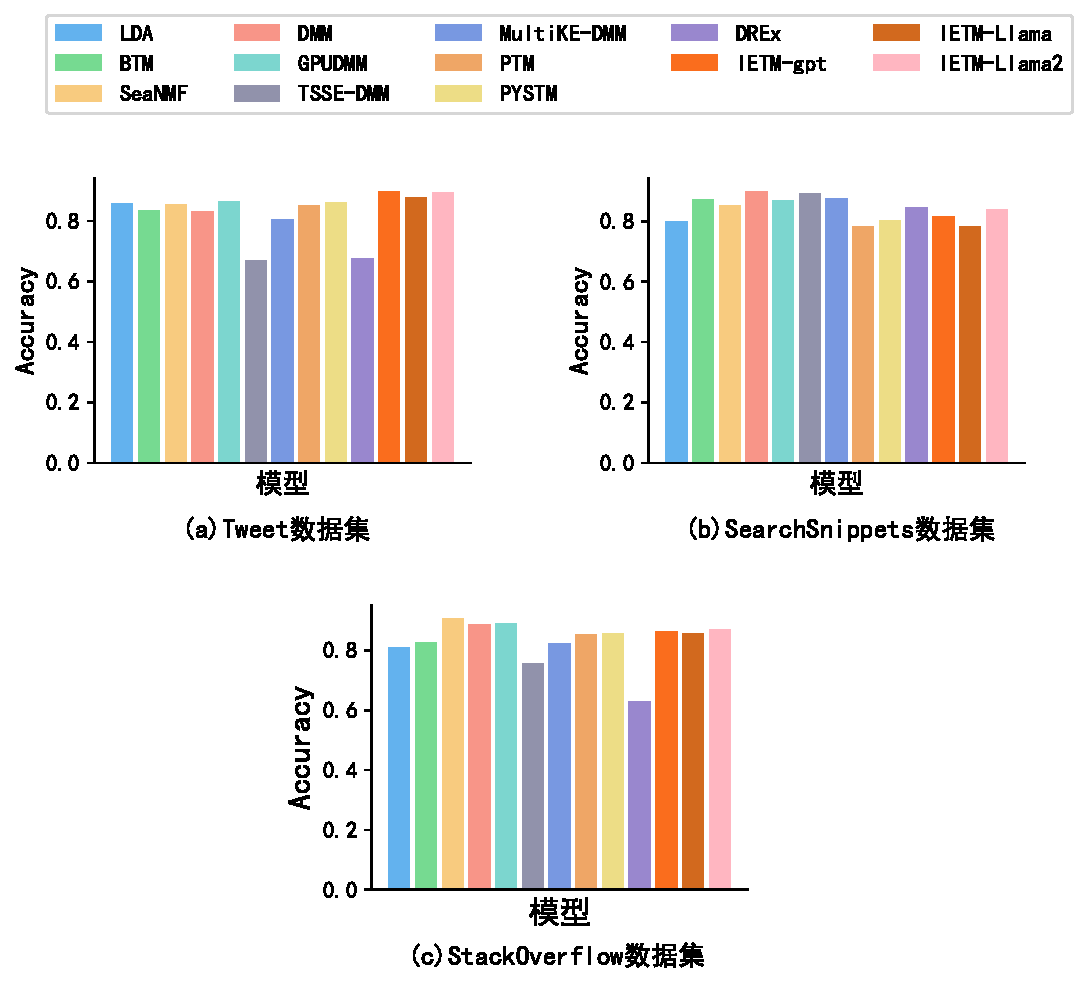
\includegraphics[width=0.85\textwidth]{chap3/Accuracy Chart.pdf}
    \caption{三个数据集的分类准确率结果图}
    \label{AccuracyChart}
\end{figure}

使用线性核支持向量机(SVM),实验在三个数据集上进行了5折交叉验证并记录平均准确率得分。具体来说,使用不同模型学习到的主题分布作为特征,并训练SVM分类器来预测每个短文本的类别。图\ref{AccuracyChart}显示,我们提出的TPTM在Tweet和StackOverflow数据集中的表现高于平均水平。然而,在SearchSnippets数据集中,TPTM无法与基线模型相比达到竞争性能。其表现不佳的一个可能原因是SearchSnippets并非严格意义上的短文本.对于Instructed-Expansion而言,这可能会导致LLMs引入不相关的语义信息。鉴于SearchSnippets数据集中只有8个类别,另一个原因可能是基于DMM的模型中使用的假设,即一个文档只关注一个主题,这对于分类任务来说更为合适。此外,可以观察到没有模型在所有数据集中都具有绝对优势。类似的结果可以在\cite{STTM}中找到。总之,我们模型学习到的主题分布具有辨别力,因此可以用于短文本分类的下游任务。

\subsection{消融实验}
如果只考虑TPTM的第一阶段,TPTM将退化为标准的LDA模型,这意味着使用LDA模型直接建模扩展后的伪文档。在本节中,我们主要讨论,与单纯使用伪文档进行LDA建模相比,通过TPTM联合建模原始文档和伪文档的有效性。本节对IE-GPT、IE-llama和IE-llama2获得的伪文档语料库使用LDA进行建模,分别命名为LDA-GPT、LDA-llama和LDA-llama2,并设定$\alpha=1.0$ 和 $\beta=0.01$。在$K=50$的条件下的结果呈现在表\ref{TableModelValidityTweet}中,其中最佳值以粗体显示。对于所有指标,本节进行了$t$检验,以显示TPTM和LDA在结果平均值上的性能差异是否具有统计显著性。如果从$t$检验中得到的$P$值低于0.05,可以认为成对性能差异是显著的。TPTM-GPT在TU得分方面表现出比LDA-GPT统计上更好的表现,而在NPMI方面的下降不显著。对于TPTM-llama和TPTM-llama2,结果也是类似的。这表明,我们提出的TPTM模型在综合主题质量方面比仅使用LDA建模伪文档更优。

\begin{table}
\centering
\caption{三个数据集在LDA和TPTM下的主题质量}
\label{TableModelValidityTweet}
\adjustbox{width=0.9\textwidth}{
\begin{tabular}{lccc|ccc|ccc}
\toprule
\multicolumn{1}{c}{\multirow{2}{*}{模型}} & \multicolumn{3}{c|}{Tweet} & \multicolumn{3}{c|}{SearchSnippets} & \multicolumn{3}{c}{StackOverflow} \\
\multicolumn{1}{c}{} & NPMI & TU & TQ & NPMI & TU & TQ & NPMI & TU & TQ \\ \midrule
LDA & 0.187 & 0.872 & \multicolumn{1}{c|}{0.163} & 0.234 & 0.799 & \multicolumn{1}{c|}{0.187} & 0.212 & 0.592 & 0.126 \\
LDA-GPT & 0.227 & 0.785$\downarrow$ & \multicolumn{1}{c|}{0.178} & 0.258 & 0.816$\downarrow$ & \multicolumn{1}{c|}{0.211$\downarrow$} & \textbf{0.242} & 0.680$\downarrow$ & 0.165$\downarrow$ \\
LDA-llama & 0.219 & 0.877$\downarrow$ & \multicolumn{1}{c|}{0.192} & 0.249 & 0.954 & \multicolumn{1}{c|}{\textbf{0.238}} & 0.228 & 0.874$\downarrow$ & 0.199 \\
LDA-llama2 & \textbf{0.230} & 0.858$\downarrow$ & \multicolumn{1}{c|}{0.197$\downarrow$} & \textbf{0.266} & 0.816$\downarrow$ & \multicolumn{1}{c|}{0.217$\downarrow$} & 0.240 & 0.743$\downarrow$ & 0.178$\downarrow$ \\ \midrule
TPTM-GPT & 0.223 & 0.818 & \multicolumn{1}{c|}{0.182} & 0.252 & 0.889 & \multicolumn{1}{c|}{0.224} & \textbf{0.242} & 0.727 & 0.176 \\
TPTM-llama & 0.216 & \textbf{0.905} & \multicolumn{1}{c|}{0.195} & 0.246 & 0.965 & \multicolumn{1}{c|}{\textbf{0.237}} & 0.224 & \textbf{0.893} & \textbf{0.200} \\
TPTM-llama2 & \textbf{0.230} & 0.877 & \multicolumn{1}{c|}{\textbf{0.202}} & \textbf{0.265} & 0.878 & \multicolumn{1}{c|}{0.233} & 0.238 & 0.789 & 0.188
\\\bottomrule
\end{tabular}}
\end{table}

\begin{figure}[ht]
    \centering
    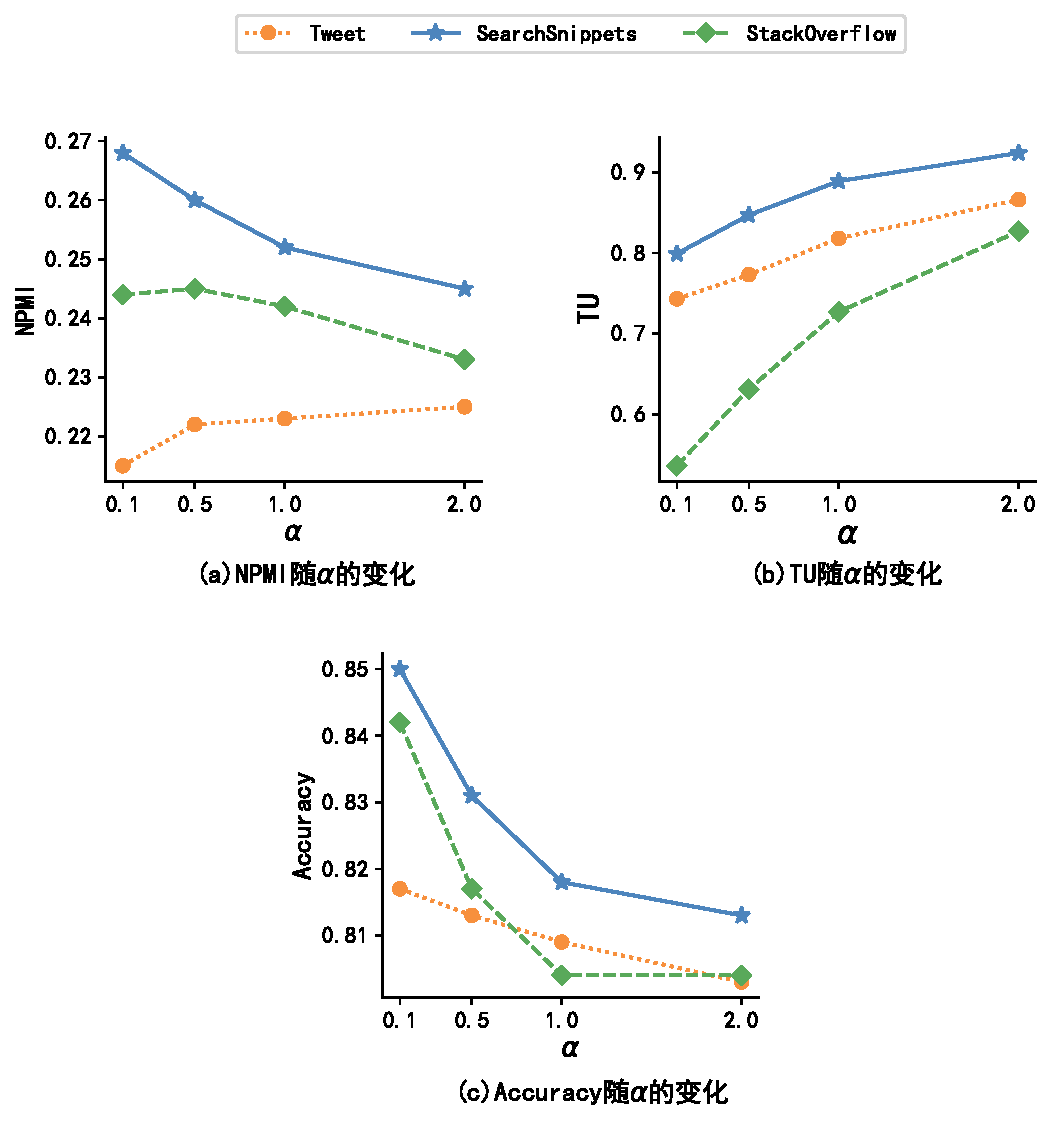
\includegraphics[width=0.8\linewidth]{chap3/resultOfAlpha.pdf}
    \caption{不同超参数值$\alpha$下的 TPTM 性能}
    \label{influenceofAlpha}
\end{figure}

\subsection{\texorpdfstring{参数$\alpha$的影响}{参数alpha的影响}}
本节在三个数据集上执行主题推断和分类任务,同时将$K$固定在50,以分析参数$\alpha$的影响。通过调整$\alpha$在${0.1, 0.5, 1, 2}$中的值,得到的结果如图\ref{influenceofAlpha}所示。总体而言,随着$\alpha$的增加,NPMI倾向于下降,而TU随着$\alpha$的增加而上升。然而,分类准确度(ACC)随着$\alpha$的增加而趋于下降。为了在主题质量和分类/聚类指标之间达到平衡,我们在上述实验中为TPTM选择了$\alpha=1.0$。

\subsection{主题展示}
本节展示了潜在主题的定性评估。以SearchSnippets数据集作为示例,因为它只包含八个类别。本节选择了与“computer”相关的主题作为示例。表\ref{Topics}展示了基线模型和TPTM挖掘出的主题示例。每个主题通过前十个词进行可视化。加粗的词表示噪音大且缺乏代表性。可以观察到这些主题聚焦于硬件、软件、操作系统、算法和网络。基线模型生成了一些具有重复词汇或主题内混淆词汇的重复主题。例如,在LDA模型得到的主题中,我们发现了一些“comedy”之类与“computer”主题无关的单词;GPU-DMM则包含“advertising”等词,并且会将细分主题网络和硬件混淆在一起;TSSE-DMM则包含许多重复且无关的单词;DREx只能挖掘出少部分与“computer”相关的词,并且也存在细分主题混淆的问题,再次验证DREx具有模糊主题之间区别的可能。相反,可以看到TPTM-llama2为对应的每个细分领域生成了一个的连贯的主题,且主题质量更高。

\section{本章小结}
在本章中,我们提出了基于提示的数据增强方法(Instructed-Expansion),以丰富短文本的词汇共现信息。此外,为了充分利用原始短文本和扩充后的伪文档,我们设计了一种新颖的方法,即基于成对文本数据的主题模型(TPTM)。在三个基准数据集上的实验表明,TPTM显著优于基线模型,有效克服了短文本的数据稀疏问题。

\begin{table}[ht]
\centering
\caption{利用各个模型从SearchSnippets数据集中挖掘的主题}
\label{Topics}
\adjustbox{width=0.9\textwidth}{
\begin{tabular}{ll}
\\\toprule
模型 & \multicolumn{1}{c}{与“computer”相关的主题示例} \\\midrule
\multirow{5}{*}{LDA} & compute parallel \textbf{comedy} \textbf{edu} \textbf{org} performance archive www http cluster \\
    & web page search home online job com dictionary definition \textbf{information} \\
    & memory intel computer chip processor apple virtual server core microsoft  \\
    & program computer language code data java tutorial web algorithm source \\
    & software system release linux download analysis project design \textbf{information} process  \\\midrule
% \multirow{5}{*}{BTM} & program java document xml instruction machine library language code web &  \\
%     & intel processor chip core amd \textbf{duo} pentium \textbf{athlon} cpu news &  \\
%     & \textbf{computer} \textbf{system} data parallel compute \textbf{edu} research information design analysis &  \\
%     & software \textbf{computer} web linux network device release security internet server &  \\
%     & memory \textbf{computer} access cache ram virtual definition disk \textbf{webopedia} \textbf{system} &  \\\midrule
\multirow{6}{*}{SeaNMF} & web search server page browser service site google website design \\
    & computer virus \textbf{memory} architecture personal \textbf{software} graphic network parallel application \\
    & program language java degree master objectoriented \textbf{tutorial} \textbf{phd} \textbf{learn} \textbf{graduate} \\
    & \textbf{software} device linux \textbf{memory} driver virtual xml disk window hardware \\
    & internet test service network connection speed bandwidth security access provider \\
    & intel processor core chip duo \textbf{pentium} amd cpu \textbf{athlon} \textbf{itanium} \\\midrule
% \multirow{5}{*}{DMM} & data algorithm \textbf{disney} system structure walt analysis consumption \textbf{consumer} design &  \\
%     & web release \textbf{software} machine instruction access \textbf{beta} wireless linux \textbf{instant} &  \\
%     & program computer \textbf{software} \textbf{wikipedia} linux driver language device web system &  \\
%     & internet network computer security bandwidth service virus test connection speed &  \\
%     & intel chip processor computer core amd cpu pentium news athlon &  \\\midrule
\multirow{5}{*}{GPUDMM} & \textbf{system} data structure xml algorithm document library respiratory analysis information \\
    & internet service share bandwidth test video connection speed \textbf{photo} \textbf{advertising} \\
    & intel memory processor chip computer amd cpu cache core virtual \\
    & computer device linux network security apple driver unix \textbf{system} virus \\
    & program web java software page computer server machine language code \\\midrule
\multirow{4}{*}{TSSE-DMM} & memory computer virtual \textbf{webopedia} cache definition \textbf{encyclopedia} \textbf{wiki} \textbf{wikipedia} web \\
    & internet network \textbf{computer} device security bandwidth access wireless \textbf{wiki} encyclopedia \\
    & programming web software java \textbf{digital} systems linux library \textbf{computer} data \\
    & intel \textbf{wiki} encyclopedia \textbf{computer} wikipedia chip software processor amd news \\\midrule
% \multirow{5}{*}{PTM}
%     & program job web java search com computer code \textbf{employment} language &  \\
%     & software management \textbf{product} system \textbf{development} tool service database engineering design &  \\
%     & computer network \textbf{digital} internet web apple \textbf{camera} \textbf{review} access wireless &  \\
%     & memory degree master virtual julia robert \textbf{graduation} cache ram \textbf{picasso} &  \\
%     & intel chip processor cpu core amd budget \textbf{pentium} \textbf{fund} athlon &  \\\midrule
\multirow{5}{*}{PYSTM} & intel chip processor amd core apple \textbf{pentium} consumption nanotechnology athlon \\
    & computer memory virtual linux operating system disk windows cache architecture \\
    & parallel computing degree \textbf{course} \textbf{thesis} master stress \textbf{phd} program \textbf{edu} \\
    & programming software java code web language source descartes release developer \\
    & server machine instruction \textbf{hypotheses} client cabinet spam web virus spyware \\\midrule
\multirow{3}{*}{DREx} 
    & network access service system security mobile computer social internet personal \\
    & computer device digital cell desktop mobile hardware intel flash memory \\
    & system information process solution product resource data management tool strategy \\\midrule
\multirow{5}{*}{TPTM-llama2} & computer memory compute virtual performance intel processor parallel chip architecture \\
    & system software device design user linux code developer download tool \\
    & data process model method analysis tool approach structure application algorithm \\
    & internet share network access user platform medium communication connect message \\
    & home web website page welcome server visit client homepage http www \\\bottomrule
\end{tabular}
}
\end{table}

